\documentclass{standalone}
\usepackage{tikz}
\usetikzlibrary{patterns, positioning}


\begin{document}
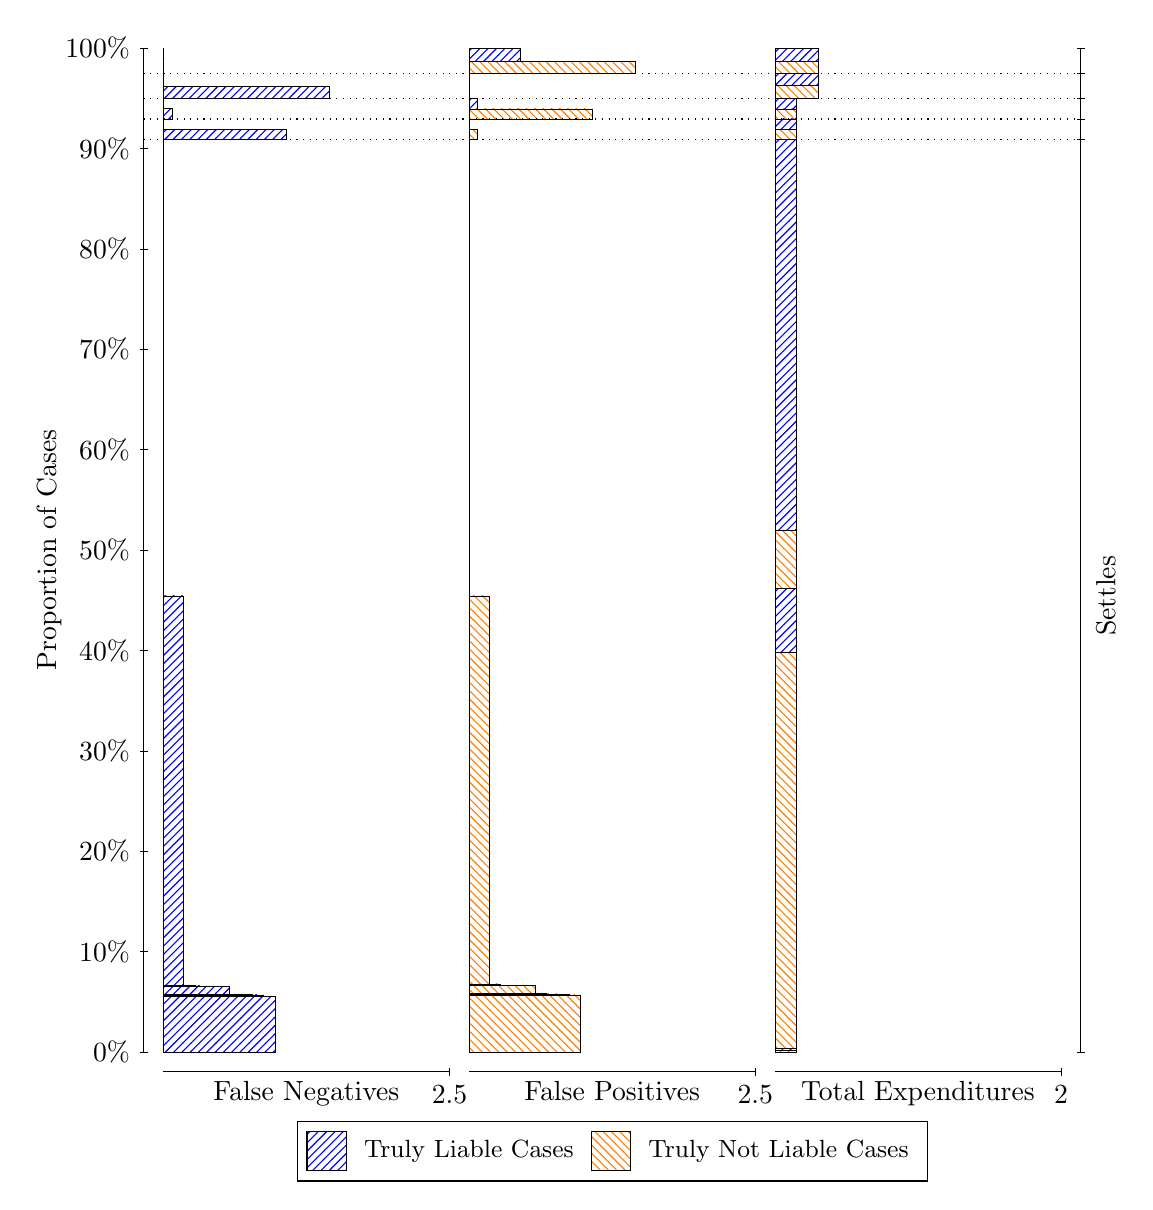
\begin{tikzpicture}
\draw[black, very thin] (1.5,1.75) -- (1.5,14.5);
\node[rotate=90, text=black, anchor=center] at (0.3, 8.125) {Proportion of Cases};
\draw[black, very thin] (1.45,1.75) -- (1.55,1.75);
\node[text=black, anchor=east] at (1.45, 1.75) {0\%};
\draw[black, very thin] (1.45,3.025) -- (1.55,3.025);
\node[text=black, anchor=east] at (1.45, 3.025) {10\%};
\draw[black, very thin] (1.45,4.3) -- (1.55,4.3);
\node[text=black, anchor=east] at (1.45, 4.3) {20\%};
\draw[black, very thin] (1.45,5.575) -- (1.55,5.575);
\node[text=black, anchor=east] at (1.45, 5.575) {30\%};
\draw[black, very thin] (1.45,6.85) -- (1.55,6.85);
\node[text=black, anchor=east] at (1.45, 6.85) {40\%};
\draw[black, very thin] (1.45,8.125) -- (1.55,8.125);
\node[text=black, anchor=east] at (1.45, 8.125) {50\%};
\draw[black, very thin] (1.45,9.4) -- (1.55,9.4);
\node[text=black, anchor=east] at (1.45, 9.4) {60\%};
\draw[black, very thin] (1.45,10.675) -- (1.55,10.675);
\node[text=black, anchor=east] at (1.45, 10.675) {70\%};
\draw[black, very thin] (1.45,11.95) -- (1.55,11.95);
\node[text=black, anchor=east] at (1.45, 11.95) {80\%};
\draw[black, very thin] (1.45,13.225) -- (1.55,13.225);
\node[text=black, anchor=east] at (1.45, 13.225) {90\%};
\draw[black, very thin] (1.45,14.5) -- (1.55,14.5);
\node[text=black, anchor=east] at (1.45, 14.5) {100\%};

\draw[black, very thin] (13.4,1.75) -- (13.4,14.5);
\draw[black, very thin] (13.35,1.75) -- (13.45,1.75);
\node[anchor=west] at (13.35, 1.75) {};
\draw[black, very thin] (13.35,13.336) -- (13.45,13.336);
\node[anchor=west] at (13.35, 13.336) {};
\draw[black, very thin] (13.35,13.599) -- (13.45,13.599);
\node[anchor=west] at (13.35, 13.599) {};
\draw[black, very thin] (13.35,13.862) -- (13.45,13.862);
\node[anchor=west] at (13.35, 13.862) {};
\draw[black, very thin] (13.35,14.181) -- (13.45,14.181);
\node[anchor=west] at (13.35, 14.181) {};
\draw[black, very thin] (13.35,14.5) -- (13.45,14.5);
\node[anchor=west] at (13.35, 14.5) {};

\draw[black, very thin, pattern color=blue, pattern=north east lines] (1.75,1.75) rectangle (3.167,2.4609);
\draw[black, very thin, pattern color=blue, pattern=north east lines] (1.75,2.4609) rectangle (3.0217,2.4756);
\draw[black, very thin, pattern color=blue, pattern=north east lines] (1.75,2.4756) rectangle (2.8763,2.48);
\draw[black, very thin, pattern color=blue, pattern=north east lines] (1.75,2.48) rectangle (2.731,2.4814);
\draw[black, very thin, pattern color=blue, pattern=north east lines] (1.75,2.4814) rectangle (2.5857,2.5839);
\draw[black, very thin, pattern color=blue, pattern=north east lines] (1.75,2.5839) rectangle (2.4403,2.5869);
\draw[black, very thin, pattern color=blue, pattern=north east lines] (1.75,2.5869) rectangle (2.295,2.5895);
\draw[black, very thin, pattern color=blue, pattern=north east lines] (1.75,2.5895) rectangle (2.1497,2.6006);
\draw[black, very thin, pattern color=blue, pattern=north east lines] (1.75,2.6006) rectangle (2.0043,7.5432);
\draw[black, very thin, pattern color=orange, pattern=north west lines] (1.75,7.5432) rectangle (1.75,13.336);
\draw[black, very thin, pattern color=blue, pattern=north east lines] (1.75,13.336) rectangle (3.3123,13.464);
\draw[black, very thin, pattern color=orange, pattern=north west lines] (1.75,13.464) rectangle (1.75,13.599);
\draw[black, very thin, pattern color=blue, pattern=north east lines] (1.75,13.599) rectangle (1.859,13.734);
\draw[black, very thin, pattern color=orange, pattern=north west lines] (1.75,13.734) rectangle (1.75,13.862);
\draw[black, very thin, pattern color=blue, pattern=north east lines] (1.75,13.862) rectangle (3.8573,14.012);
\draw[black, very thin, pattern color=orange, pattern=north west lines] (1.75,14.012) rectangle (1.75,14.181);
\draw[black, very thin, pattern color=orange, pattern=north west lines] (1.75,14.181) rectangle (1.75,14.331);
\draw[black, very thin, pattern color=blue, pattern=north east lines] (1.75,14.331) rectangle (1.75,14.5);
\draw[black, very thin, pattern color=orange, pattern=north west lines] (5.6333,1.75) rectangle (7.0503,2.4749);
\draw[black, very thin, pattern color=orange, pattern=north west lines] (5.6333,2.4749) rectangle (6.905,2.4848);
\draw[black, very thin, pattern color=orange, pattern=north west lines] (5.6333,2.4848) rectangle (6.7597,2.4871);
\draw[black, very thin, pattern color=orange, pattern=north west lines] (5.6333,2.4871) rectangle (6.6143,2.4898);
\draw[black, very thin, pattern color=orange, pattern=north west lines] (5.6333,2.4898) rectangle (6.469,2.5926);
\draw[black, very thin, pattern color=orange, pattern=north west lines] (5.6333,2.5926) rectangle (6.3237,2.5927);
\draw[black, very thin, pattern color=orange, pattern=north west lines] (5.6333,2.5927) rectangle (6.3237,2.5942);
\draw[black, very thin, pattern color=orange, pattern=north west lines] (5.6333,2.5942) rectangle (6.1783,2.5991);
\draw[black, very thin, pattern color=orange, pattern=north west lines] (5.6333,2.5991) rectangle (6.033,2.6156);
\draw[black, very thin, pattern color=orange, pattern=north west lines] (5.6333,2.6156) rectangle (5.8877,7.5429);
\draw[black, very thin, pattern color=blue, pattern=north east lines] (5.6333,7.5429) rectangle (5.6333,13.336);
\draw[black, very thin, pattern color=orange, pattern=north west lines] (5.6333,13.336) rectangle (5.7423,13.471);
\draw[black, very thin, pattern color=blue, pattern=north east lines] (5.6333,13.471) rectangle (5.6333,13.599);
\draw[black, very thin, pattern color=orange, pattern=north west lines] (5.6333,13.599) rectangle (7.1957,13.727);
\draw[black, very thin, pattern color=blue, pattern=north east lines] (5.6333,13.727) rectangle (5.7423,13.862);
\draw[black, very thin, pattern color=orange, pattern=north west lines] (5.6333,13.862) rectangle (5.6333,14.031);
\draw[black, very thin, pattern color=blue, pattern=north east lines] (5.6333,14.031) rectangle (5.6333,14.181);
\draw[black, very thin, pattern color=orange, pattern=north west lines] (5.6333,14.181) rectangle (7.7407,14.331);
\draw[black, very thin, pattern color=blue, pattern=north east lines] (5.6333,14.331) rectangle (6.2873,14.5);
\draw[black, very thin, pattern color=orange, pattern=north west lines] (9.5167,1.75) rectangle (9.7892,1.773);
\draw[black, very thin, pattern color=blue, pattern=north east lines] (9.5167,1.773) rectangle (9.7892,1.7935);
\draw[black, very thin, pattern color=orange, pattern=north west lines] (9.5167,1.7935) rectangle (9.7892,6.8236);
\draw[black, very thin, pattern color=blue, pattern=north east lines] (9.5167,6.8236) rectangle (9.7892,7.637);
\draw[black, very thin, pattern color=orange, pattern=north west lines] (9.5167,7.637) rectangle (9.7892,8.3768);
\draw[black, very thin, pattern color=blue, pattern=north east lines] (9.5167,8.3768) rectangle (9.7892,13.336);
\draw[black, very thin, pattern color=orange, pattern=north west lines] (9.5167,13.336) rectangle (9.7892,13.471);
\draw[black, very thin, pattern color=blue, pattern=north east lines] (9.5167,13.471) rectangle (9.7892,13.599);
\draw[black, very thin, pattern color=orange, pattern=north west lines] (9.5167,13.599) rectangle (9.7892,13.727);
\draw[black, very thin, pattern color=blue, pattern=north east lines] (9.5167,13.727) rectangle (9.7892,13.862);
\draw[black, very thin, pattern color=orange, pattern=north west lines] (9.5167,13.862) rectangle (10.062,14.031);
\draw[black, very thin, pattern color=blue, pattern=north east lines] (9.5167,14.031) rectangle (10.062,14.181);
\draw[black, very thin, pattern color=orange, pattern=north west lines] (9.5167,14.181) rectangle (10.062,14.331);
\draw[black, very thin, pattern color=blue, pattern=north east lines] (9.5167,14.331) rectangle (10.062,14.5);
\draw[black, dotted] (1.5,13.336) -- (13.4,13.336);
\draw[black, dotted] (1.5,13.599) -- (13.4,13.599);
\draw[black, dotted] (1.5,13.862) -- (13.4,13.862);
\draw[black, dotted] (1.5,14.181) -- (13.4,14.181);
\draw[black, very thin] (1.75,1.5) -- (5.3833,1.5);
\node[text=black, anchor=north] at (3.5667, 1.5) {False Negatives};
\draw[black, very thin] (5.3833,1.45) -- (5.3833,1.55);
\node[text=black, anchor=north] at (5.3833, 1.45) {2.5};

\draw[black, very thin] (5.6333,1.5) -- (9.2667,1.5);
\node[text=black, anchor=north] at (7.45, 1.5) {False Positives};
\draw[black, very thin] (9.2667,1.45) -- (9.2667,1.55);
\node[text=black, anchor=north] at (9.2667, 1.45) {2.5};

\draw[black, very thin] (9.5167,1.5) -- (13.15,1.5);
\node[text=black, anchor=north] at (11.333, 1.5) {Total Expenditures};
\draw[black, very thin] (13.15,1.45) -- (13.15,1.55);
\node[text=black, anchor=north] at (13.15, 1.45) {2};

\node[text=black, centered, rotate=90] at (13.72, 7.543) {Settles};





\draw (7.449999999999999,1.5) node[draw=none] (baseCoordinate) {};
\begin{scope}[align=center]
        \matrix[scale=0.5, draw=black, below=0.5cm of baseCoordinate, nodes={draw}, column sep=0.1cm]{
            \node[rectangle, draw, minimum width=0.5cm, minimum height=0.5cm, pattern color=blue, pattern=north east lines] {}; &
            \node[draw=none, font=\small, text=black] (B) {Truly Liable Cases}; &
            \node[rectangle, draw, minimum width=0.5cm, minimum height=0.5cm, pattern color=orange, pattern=north west lines] {}; &
            \node[draw=none, font=\small, text=black] (B) {Truly Not Liable Cases}; \\
            };
\end{scope}

\end{tikzpicture}
\end{document}